\documentclass{itatnew}
%% !!!dolezite: ak pisete po slovensky alebo po cesky pouzite
%% \documentclass[slovensky]{itatnew}
%% \documentclass[cesky]{itatnew}

% Math shortcuts
\usepackage{amssymb}
\usepackage{algorithm}
\usepackage{algorithmic}
\newcommand{\xx}{\mathrm{\mathbf{x}}}
\newcommand{\yy}{\mathrm{\mathbf{y}}}
\newcommand{\XX}{\mathrm{\mathbf{X}}}
\newcommand{\CC}{\mathrm{\mathbf{C}}}
\newcommand{\ttheta}{\mathbf{\theta}}
\newcommand{\eell}{\boldsymbol\ell}
% \newcommand{\msf}[1]{\mathsf{\mathbf{#1}}}

\begin{document}

\title{Sampling Methods for Model Guided Sampling Optimization
  with Gaussian Processes}

\author{Lukáš Bajer\inst{1,2} \and Martin Holeňa\inst{2} \and Viktor Charypar \inst{3}}

\institute{Faculty of Mathematics and Physics, Charles University in Prague,\\
Malostranské nam. 25, 118 00 Prague 1, Czech Republic \\
\email{bajer@cs.cas.cz} \\
\and
Institute of Computer Science, Academy of Sciences of the Czech Republic,\\
Pod Vodárenskou věží 2, 182 07 Prague 8, Czech Republic \\
\email{martin@cs.cas.cz} \\
\and
Faculty of Nuclear Sciences and Physical Engineering, Czech Technical University in Prague, \\
Trojanova 13, 120 00 Prague 2, Czech Republic \\
\email{charyvik@fjfi.cvut.cz} }

\maketitle              % typeset the title of the contribution

\begin{abstract}
Model Guided Sampling Optimization (MGSO) was recently proposed as an alternative for Jones' Kriging-based EGO algorithm for optimization of expensive black-box functions. Instead of maximizing a chosen criterion (e.g. expected improvement), MGSO samples probability of improvement forming multiple candidates -- a~whole population of suggested solutions. This paper tackles problems with such sampling, it compares different sampling methods and brings a new version of the MGSO algorithm.
\end{abstract}

\section{Introduction}
%
Optimization of expensive empirical functions forms an important topic in many engineering or natural-sciences areas. For such functions, it is often impossible to obtain any derivatives or information about smoothness; moreover, there is no mathematical expression nor algorithm to evaluate. Instead, some simulation or experiment has to be performed, and the measured value or result of such experiment is the value of the objective function being considered. Such functions are also called black-box functions. 
% Such empirical functions 
They are usually very expensive to evaluate; one evaluation may cost a lot of time and money to process.

Because of the absence of the derivatives, standard continuous first- or second-order derivative optimization methods cannot be used. Further, functions of this kind are usually characterized by a high number of local optima where simple algorithms can be trapped easily. Therefore, different derivative-free optimization methods for black-box functions (often called meta-heuristics) have been evolved. Even though these methods are slow and computational intensive, the cost of the evaluation of the empirical objective function is always much higher, and so the number of function evaluations is the parameter which is crucial to decrease as much as possible.
% and the cost of these evaluations dominates the computational cost of the optimization algorithm.

Evolutionary algorithms constitute a broad family of meta-heuristics that are used for black-box optimization very frequently. Some kinds of these algorithms or some techniques are designed to spent for the optimization as few objective function evaluations as possible -- all of the three following approaches use some kind of model being built and updated within the optimization process.

\emph{Estimation of distribution algorithms} (EDAs) \cite{larranaga_estimation_2002} represent one such approach: EDAs iteratively estimate the probabilistic distribution of selected candidate solutions (usually better than some threshold) and sample this distribution forming a new set of solutions for the next iteration. 

\emph{Surrogate modelling} is a technique of construction and usage of a regression model of the objective function~\cite{jin_comprehensive_2005}. The model (called surrogate model in this context) is then used to evaluate some of the candidate solutions instead of evaluating them with the original costly function.

Our method, \emph{Model Guided Sampling Optimization} (MGSO), is based on both these approaches. It is similar to Jones' Efficient Global Optimization (EGO)~\cite{jones_efficient_1998}: like EGO, MGSO uses a Gaussian process (GP, see~\cite{rasmussen_gaussian_2006} for reference), which provides a guide where to sample new candidate solutions in order to explore new solutions and exploit promising areas of the objective-function landscape. EGO evaluates a solution where a chosen criterion, Expected Improvement (EI) or Probability of Improvement (PoI) is maximized. Hennig in his recent work~\cite{hennig_entropy_2012} examines more criteria in detail. On the other hand, MGSO samples GP model's latter criterion -- PoI, producing a set of new points. At the same time, the GP serves as a surrogate model of the objective function for some of the solutions. During each iteration, MGSO samples the model's PoI forming a population of new candidate solutions, evaluates them and updates the GP model with the new gathered data.

This paper follows up to the previous brief introduction of MGSO~\cite{bajer_model_2013}. Instead of Gibbs' sampling, it uses slice sampling introduced by Neal~\cite{neal_slice_2003} which enables computationally cheaper sampling in higher dimensions. Further, the GP model is used as a surrogate model more often which brings faster convergence. The following section introduces methods used in the MGSO, Section \ref{sec:mgso} describes the MGSO algorithm and the Section \ref{sec:results} brings some preliminary results on the BBOB testing set~\cite{hansen_real_2009}.


\section{Involved Methods}

\subsection{Gaussian Processes}

Gaussian process~\cite{rasmussen_gaussian_2006} is a probabilistic model based on Gaussian distributions. 
% It is specified by covariance and mean function and relatively small number of hyper-parameters. 
It is specified by mean and covariance functions and relatively small number of covariance function's hyper-parameters. 
% The hyper-parameters are set in such way that the likelihood of the function value given the values of the decision variables is maximized for the training data points.
The hyper-parameters are set by the maximum-likelihood method.

The GP model can predict the function value in a new point in the form of univariate Gaussian distribution: the GP provides mean and the standard deviation of the function value. Through the predicted mean, the GP can serve as a surrogate model, and standard deviation is a measure of uncertainty of the prediction in a specified point.

Let $\XX_N = \{\xx_i \ | \ \xx_i \in \mathbb{R}^{D}\}_{i=1}^{N}$ be a set of $N$ training $D$-dimensional data points with known dependent-variable values $\yy = \{y_i\}_{i=1}^{N}$ and $f(\xx)$ be an unknown function being modelled for which $f(\xx_i) = y_i$ for all $i \in \{1,\ldots,N\}$. The GP model imposes a probabilistic model on the data: the vector of known function values $\yy_N$ is considered as one sample of a $N$-dimensional multivariate Gaussian distribution with probability density $p(\yy \, | \, \XX_N)$. If we add a new data point $(\xx_{N+1}, y_{N+1})$, the probability density is, according to B\"{u}che \cite{buche_accelerating_2005},
\begin{equation}
p(\yy_{N+1} \, | \, \XX_{N+1}) = \frac { \exp(-\frac{1}{2} \yy^\top_{N+1} \CC^{-1}_{N+1} \yy_{N+1}) } { \sqrt{(2\pi)^{N+1} \det(\CC_{N+1})} }
\end{equation}
where $\CC_{N+1}$ is the covariance matrix of the Gaussian distribution (for which mean is usually set to constant zero). This covariance can be written as
\begin{equation}
\CC_{N+1} = \left( \begin{array}{cc} \CC_N & \mathbf{k} \\ \mathbf{k}^\top & \kappa \end{array} \right)
\end{equation}
where $\CC_N$ is the covariance of the Gaussian distribution given the $N$ training data points, $\mathbf{k}$ is a vector containing covariances between the new point and training data, and $\kappa$ is the variance of the new point itself. Further, inverse $\CC^{-1}_{N-1}$ of the extended covariance can be expressed using inverse of the training covariance $\CC^{-1}_N$ which simplifies density of the distribution in a new point to a univariate Gaussian with density
\begin{equation}
p(y_{N+1} \, | \, \XX_{N+1}, \yy_N) \ \varpropto \ \exp \left( -\frac{1}{2} \frac {(y_{N+1} - \hat{y}_{N+1})^2} {\sigma^2_{y_{N+1}}} \right)
\label{univariate-density}.
\end{equation}
with mean and variance given by
\begin{eqnarray}
\hat{y}_{N+1} & = & \mathbf{k}^\top \CC^{-1}_N \yy_N, \\
\sigma^2_{y_{N+1}} & = & \kappa - \mathbf{k}^\top \CC^{-1}_N \mathbf{k}.
\end{eqnarray}
Further details can be found in \cite{buche_accelerating_2005}.

The covariances $\CC_N$ plays a crucial role in these equations. Gaussian processes use parametrized covariance functions $C$ describing prior assumptions on the shape of the modeled function. The covariance between the function values at two data points $\xx_p$ and $\xx_q$ is given by $C(\xx_p, \xx_q)$ which forms also the $(p,q)$-th element of the matrix $\CC_N$. In our case, we used the most common squared-exponential function
\begin{equation}
C(\xx_p, \xx_q) = \theta_1 \exp \left( -\frac{1}{2} \sum^D_{i=1} \frac{(x^i_p - x^i_q)^2} {2l^2} \right) + \theta_2 + \delta_{p,q}\theta_3
\end{equation}
which is suitable when the modelled function is rather smooth. The closer the points $\xx_p$ and $\xx_q$ are, the closer the covariance function value is to 1 and the stronger correlation between function values $f(\xx_p)$ and $f(\xx_q)$ is. The hyper-parameter $\theta_1$ scales this correlation, $\theta_2$ rises the value from zero and $\theta_3$ means a white noise of the diagonal elements of the matrix. The last parameter $l$ is the length-scale with which the distance of two considered data points is compared. Estimate of these hyper-parameters can be supplied by the user and the final value is usually learnt using maximum-likelihood approach.


\subsection{Sampling}

The core of the MGSO algorithm is made by sampling of the probability of improvement. This measure is, for a chosen threshold $T$ of the function value, directly given by the predicted mean $\hat{f}(\xx) = \hat{y}$ and the standard deviation $\hat{\sigma}(\xx) = \sigma_{y}$ of the GP model $\hat{f}$ in any point $\xx$ of the input space
\begin{equation}
  \mathrm{PoI}_T(\xx) = \mathrm{\Phi}\left( \frac{T - \hat{f}(\xx)}{\hat{\sigma}(\xx)} \right) = \mathrm{P}(\hat{f}(\xx) \leqq T)
\end{equation}
which corresponds to the value of cumulative distribution function (CDF) of the Gaussian with already mentioned density (\ref{univariate-density}). Even though all the variables come from Gaussian distribution, $\mathrm{PoI}(\xx)$ is definitely not Gaussian-shaped since it depends on the threshold $T$ and the function being modeled $f$ -- typical example of the landscape of $\textrm{PoI}(\xx)$ in two dimensions for Rastrigin function is depicted in Fig.\,1 % THIS DOES NOT WORK :( \ref{fig:poi}.
The dependency on the modelled function causes also no analytical marginals, derivatives or conditional probabilities of this density.

\begin{figure}
  \centering
  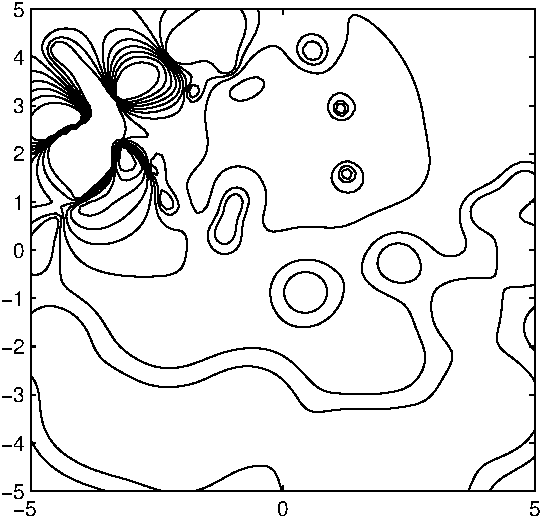
\includegraphics[width=0.6\linewidth]{poi_example}
  {\small
  \caption{Probability of improvement. Rastrigin function in 2D, GP model built with 40 data points.
  \label{fig:poi}
  }
  }
\end{figure}

\paragraph{Gibbs' sampler.}

The first version of MGSO~\cite{bajer_model_2013} used Gibbs' sampler~\cite{geman_stochastic_1984}. The sampler starts at some point of the input space $\xx_s$. Further, it moves along each dimension to a new point $\xx'$: it cycle successively through each individual dimension $k = 1,\ldots,D$ by assessing its value through sampling from conditional probability of this variable given values of the remaining ones: for $k=1,\ldots,D$
\begin{equation}
X^k \sim p(X^k \, | \, \{X^j = x^j, j \neq k)\}).
\end{equation}
As no analytical expression for these conditionals exists, inverse of the empirical conditional CDF's $F^{-1}_k$ was used to transform samples from uniform distributions
\begin{displaymath}
u^k \sim U(0,1), \quad  x^k = F^{-1}_k(u_k).
\end{displaymath}
Linear interpolation between values of the empirical CDF was computed at the 20-points grid.

Even though evaluating GP model's mean $\hat{y} = \hat{f}(\xx)$ and standard deviation $\hat{\sigma}(\xx)$ for 20 points requires only two calls of GP model prediction, the complexity of sampling rises quickly with the number of variables $D$ which causes sampling in more than three dimensions being extremely slow.

\paragraph{Slice sampling.}

\begin{algorithm}[b]
\begin{algorithmic}[1]
{\small
\STATE \textbf{Input}: $f$ -- function proportional to the density \\
  \quad $\xx_0$ -- starting point, $\xx_0 \in \mathbb{R}^D$ \\
  \quad $\mathbf{w}$ -- scale estimates, $\mathbf{w} \in \mathbb{R}^D$ \\
  \quad $n$ -- required number of samples
\FOR {$k = 0,1,\ldots,n$}
  % \STATE \COMMENT{define the slice} \\
  \STATE $y \sim U(0, \, f(\xx_k))$  \hspace{\fill}  \COMMENT{height of the slice}
  % \STATE \COMMENT{random position of the hyper-rectangle} \\
  \STATE $\mathbf{u} \sim U(0,1)^D$ %  \hspace{\fill}  \COMMENT{random shift of hyper-rectangle}
  \STATE $\mathbf{L} \leftarrow \xx_k - \mathbf{w} \circ \mathbf{u}$  \hspace{\fill}  \COMMENT{randomly shifted lower bound} % \COMMENT{$\circ$ is entrywise product}
  \STATE $\mathbf{R} \leftarrow \mathbf{L} + \mathbf{w}$   \hspace{\fill}  \COMMENT{upper bound}
  % \STATE $\mathbf{L},\mathbf{R} \leftarrow$ lower/upper bounds of a hyper-rectangle $\mathbf{H}$ \\
  % \quad $\xx_k \in \mathbf{H}, \quad R_j - L_j = w_j \ \forall j = 1,\ldots,D$
  \WHILE {given number of tries has not exceeded}
    \STATE $\mathbf{u} \sim U(0,1)^D$
    \STATE $\xx_{k+1} \leftarrow \mathbf{L} + \mathbf{u} \circ (\mathbf{R} - \mathbf{L})$ \hspace{\fill}  \COMMENT{$\xx_{k+1} \sim U(\mathbf{L},\mathbf{R})^D$}
    % \STATE $\xx_{k+1} \leftarrow$ random sample from the hyper-rectangle $[\mathbf{L}, \mathbf{R}]$
    \IF {$(y < f(\xx_{k+1}))$}
      \STATE accept $\xx_{k+1}$ and exit the \emph{while} loop
    \ENDIF
    \FOR {each dimension $j = 1,\ldots,D$}
      \IF {$(x^j_{k+1} < x^j_k)$}
      \STATE $L^j \leftarrow x^j_{k+1}$  \hspace{\fill}  \COMMENT{shrink the lower bound}
      \ELSE
      \STATE $R^j \leftarrow x^j_{k+1}$  \hspace{\fill}  \COMMENT{shrink the upper bound}
      \ENDIF
    \ENDFOR
  \ENDWHILE
\ENDFOR
\STATE \textbf{Output}: $\{\xx_1,\ldots,\xx_n\}$
}
\end{algorithmic}
\caption{Slice sampling~\cite{neal_slice_2003}}
\label{alg:slice}
\end{algorithm}

This novel kind of sampling brought by Neal~\cite{neal_slice_2003} is based on a simple and smart idea. It starts from a starting point $(\xx_0, f(\xx_0))$ where a uniform sample $y \sim U(0,f(\xx_0))$ is obtained. This number induces a subset $S=\{\xx \in \mathbb{R}^D \,|\, f(\xx) > y\}$ which is stepwise approximated by a hyper-rectangle and uniformly sampled, forming a new point $\xx_1$. The approximation of the subset is dependent on the only parameter of this method, scale estimate $\mathbf{w} \in \mathbb{R}^D$, which does not affect correctness and its wrong guess decreases the speed of convergence only moderately. The sampler then starts again from the $(\xx_1, f(\xx_1))$ and continuously generates next points, see the pseudo-code in Alg.\,\ref{alg:slice}.

Slice sampling has several advantages. First, it nicely scales with higher dimensionalities of the problem. Second, there is no need of conditional distributions as it is with Gibbs' sampler. Moreover, it does not require the density being normalized, which is the case of PoI. This kind of sampler is used in the second version of MGSO, described in this paper.


\section{Model Guided Sampling Optimization}
\label{sec:mgso}

As it was already mentioned, the MGSO algorithm for black-box optimization has many common aspects with Jones'~\cite{jones_efficient_1998} Efficient Global Optimization algorithm. Like some of the versions of EGO, it uses the probability of improvement $\mathrm{PoI}_T^{\mathsf{M}_i}(\xx)$ as a measure how promising the specified point $\xx$ is for locating the optimum given a chosen threshold $T$ and the current knowledge of the function landscape
% saved in the current dataset $\mathsf{S}_i$ and
modelled by the actual GP model $\mathsf{M}_i$. The main difference is that it does not maximizes this criterion, but it samples the PoI (which is proportional to a density) producing the whole population of individuals. 

After the initial (usually uniform random) sample of the input space, its evaluation and saving to the dataset $\mathsf{S}_0$, the MGSO algorithm proceeds as follows (see Alg.\,\ref{alg:mgso} for details; $\circ$ is a component-wise product of two vectors). First, a new GP model $\mathsf{M}_i$ is fitted to the actual dataset $\mathsf{S}_i$. The model predictive distribution guides the further optimization: the model's PoI is sampled forming the new population. The second version of MGSO added step 6: the last individual in the population is obtained by continuous local smooth optimization of the GP model which speeds-up the optimization process especially in the final part of the algorithm's run. The algorithm continues with evaluating the new population, a new model is fitted to this augmented dataset and the process is repeated until a stopping condition is met.

\begin{algorithm}[t]
\begin{algorithmic}[1]
{\small
  \STATE \textbf{Input}: $f$ -- objective function \\
      \quad $N', N$ -- sizes of the initial and standard population \\
      \quad $r$ -- no. of solutions for dataset restriction
  \STATE $\mathsf{S}_0 = \{(\xx_j, y_j)\}_{j=1}^{N'} \leftarrow$ generate $N'$ initial samples 
      and evaluate them % to get observed values $\{y_j\}_{j=1}^{N'}$ forming a dataset $\mathsf{S}_0 = \{(\xx_0, y_0)\}$
  \WHILE {no stopping condition is met, $i=1,2,\ldots$}
    \STATE $\mathsf{M}_i \leftarrow$ build a GP model and fit its hyper-parameters
        according to the dataset $\mathsf{S}_{i-1}$
    \STATE $\{\xx_j\}_{j=1}^{N}  \leftarrow$ sample the $\textrm{PoI}_T^{\mathsf{M}_i}(\xx)$ 
        forming $N$ new candidate solutions, optionally with different targets $T$
    \STATE $\xx_k \leftarrow$ find the minimum of the GP (by local continuous optimization) and replace the nearest solution from $\{\xx_j\}_{j=1}^{N}$ with it
    \STATE $\{y_j\}_{j=1}^N \leftarrow f(\{\xx_j\}_{j=1}^N)$  \hspace{\fill}  \COMMENT{evaluate the population} 
    \STATE $\mathsf{S}_i \leftarrow \mathsf{S}_{i-1} \cup \{(\xx_j, y_j)\}_{j=1}^N$  \hspace{\fill}  \COMMENT{augment the dataset} 
    \STATE $(\tilde{\xx}, \tilde{y}) \leftarrow \arg \min_{(\xx,y) \in \mathsf{S}_i} y$  \hspace{\fill}  \COMMENT{find the best solution in $\mathsf{S}_i$}
    \IF {any rescale condition is met} 
    \STATE restrict the dataset $\mathsf{S}_i$ to the bounding-box $[\mathbf{l}_i,\mathbf{u}_i]$ of the $r$ nearest solutions along the best solution $(\tilde{\xx},\tilde{y})$ and linearly transform $\mathsf{S}_i$ to $[-1, 1]^D$
    \ENDIF
  \ENDWHILE
  \STATE \textbf{Output}: the best found solution $(\tilde{\xx}, \tilde{y})$
}
\end{algorithmic}
\caption{MGSO (Model Guided Sampling Optimization)}
\label{alg:mgso}
\end{algorithm}

To abstract from the search space scaling, MGSO works in an internal, linearly transformed coordinate system defined by mapping
\begin{equation}
\mathit{scale}:[\mathbf{l}, \mathbf{u}] \rightarrow [-1, 1]^D
\end{equation}
and the transformation can be updated during the optimization. Updating it restricts the learning and sampling space to the neighborhood of the so-far optimum, which enables sampling in the situation when the PoI is non-zero only in a very small region. The lower and upper bounds $[\mathbf{l}_i, \mathbf{u}_i], \hspace{0.7em} \mathbf{l}_i,\mathbf{u}_i \in \mathbb{R}^D$ in each coordinate dimension are determined as a bounding box of $r$ nearest samples from the current optimum, expanded by 10\%; the default is $r=15\cdot D$. These bounds can be updated each iteration~$i$, but they are updated only several times during one optimization run in practice. The value $r$, the initial number of samples $N'$ and the population size $N$ are input parameters of MGSO.

The slice sampling method enables us to sample multivariate distributions more easily. Slice sampling from Matlab Statistical toolbox was used which implements shrinking-in of all dimensions. The sampler is extended by a validity-checking of the GP model -- the samples which addition results in ill-con\-di\-tion\-ed covariance matrix are rejected. Further, different thresholds $T$ for $\mathrm{PoI}_T^{\mathsf{M}_i}$ are tested if many such rejections arise.

\section{Experimental Results and Conclusion}
\label{sec:results}

\subsection{Sampling}

The slice sampling has shown to be a noticeable improvement both in terms of the computational resources and the ability of sample enough samples. The results for two and five dimensions are shown in Tab.\,\ref{tab:sampling}, sampling times and the numbers of really generated samples are depicted in Fig.\,\ref{fig:sampling}.

\begin{table}% [!bh]
\begin{center}
{\small
\caption{Comparison of Gibbs' and Slice sampling in 2D and 5D, results from 15 runs of sampling. Generated 20 samples in 2D and 50 samples in 5D.}
\vspace{1ex}
\label{tab:sampling}
\begin{tabular}{l | c c c c}
\hline
            & Gibbs 2D  & slice 2D      & Gibbs 5D      & slice 5D \\
\hline
time [s]    & 1.85      & 1.11          & 42.41         & 17.56 \\
\# of eval. & 2 402     & 246           & 20 087        & 2 909 \\
\hline
\end{tabular}
} % \small
% \vspace{2ex}
\end{center}
\end{table}

\begin{figure}
  \centering
  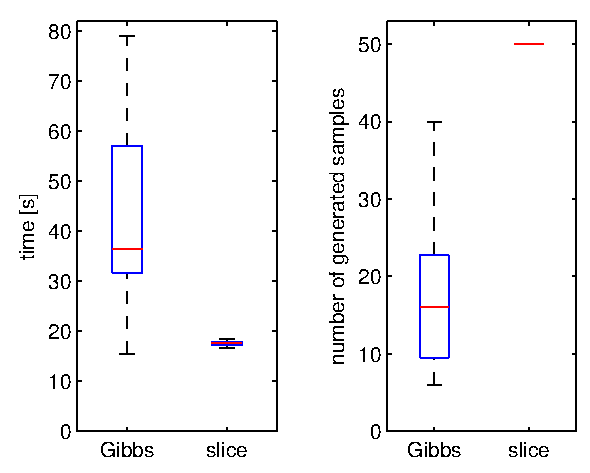
\includegraphics[width=0.9\linewidth]{sampling_time_popsize_5D}
  {\small
  \caption{Computational time and the number of really generated samples in 5D. Results from 15 independent runs with the same GP model/PoI.
  \label{fig:sampling}
  }
  }
\end{figure}

\subsection{BBOB Benchmark Functions Optimization}

The proposed MGSO has been tested on three different continuous benchmark functions from the BBOB testing set~\cite{hansen_real_2009}: sphere, Rosenbrock and Rastrigin functions. Although the previous version of the algorithm~\cite{bajer_model_2013} was practically able to optimize only two-dimensional versions of these functions, this paper provides results from 5D and 10D as well. The rapid speed-up was caused mainly by the slice sampling method and partly also by the continuous local optimization step performed every iteration.

The performance of the algorithm was compared with the Covariance Matrix Adaptation Evolution Strategy (CMA-ES)~\cite{hansen_completely_2001} -- the state-of-the art in the field of continuous black-box optimization methods. In two dimensions, the current version of the MGSO outperformed CMA-ES (considering budget 500 original evaluations) on both sphere and Rosenbrock functions, and it performs approximately equally well on Rastrigin function, see Fig.\,\ref{fig:optim_2D}.

The MGSO scales nicely on the easy sphere function. Both in 5D and 10D, dramatically lower number of function evaluations is needed to reach threshold of the objective function values $f_{\Delta} = 10^{-4}$ than in the case of CMA-ES, see Fig.\,\ref{fig:optim_5D} and Fig.\,\ref{fig:optim_10D}. On the Rosenbrock function, the number of evaluations of MGSO needed to reach $f_{\Delta} = 10^{-2}$ is lower in 5D, but CMA-ES works better in 10D. The hardest Rastrigin function with extensive number of local minima is not harder than the two other functions for CMA-ES, but it is not the case of MGSO. Our algorithm is outperformed by CMA-ES in both Rosenbrock and Rastrigin functions.


\begin{figure}
  \centering
  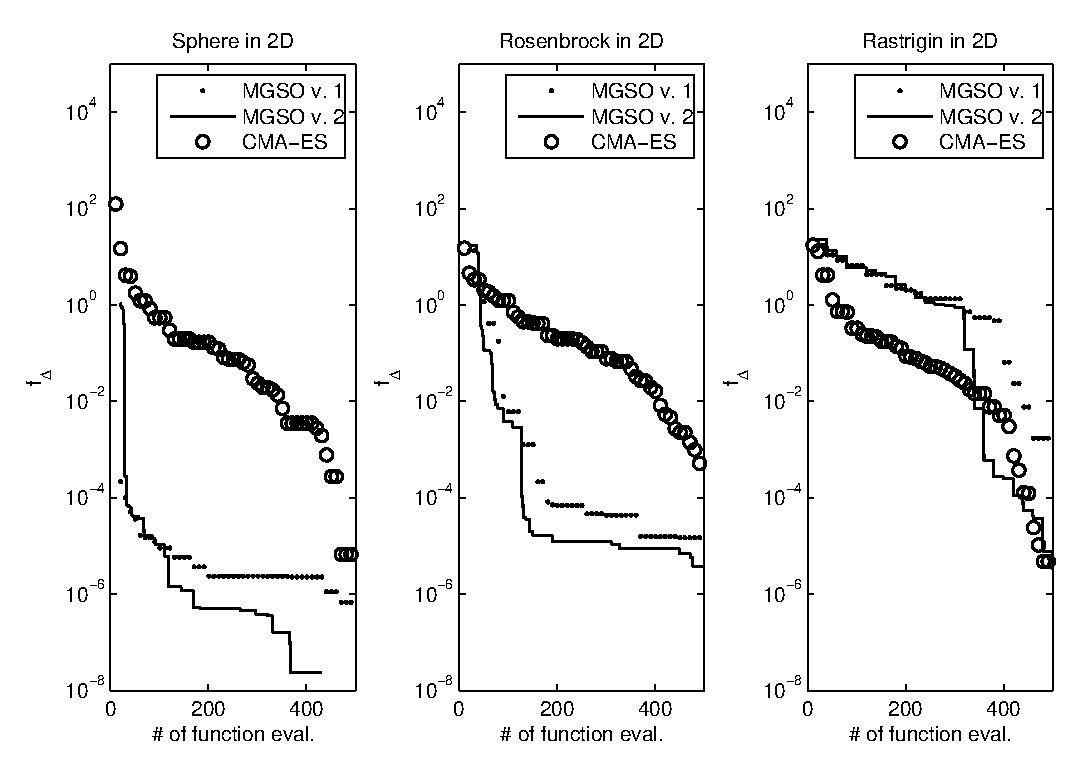
\includegraphics[width=\linewidth]{optim_2D}
  {\small
    \caption{2-D. Medians of the best found function values gathered from 15 independent runs. First~\cite{bajer_model_2013} and second version of MGSO is compared with CMA-ES.
  \label{fig:optim_2D}
  }
  }
\end{figure}


\begin{figure}
  \centering
  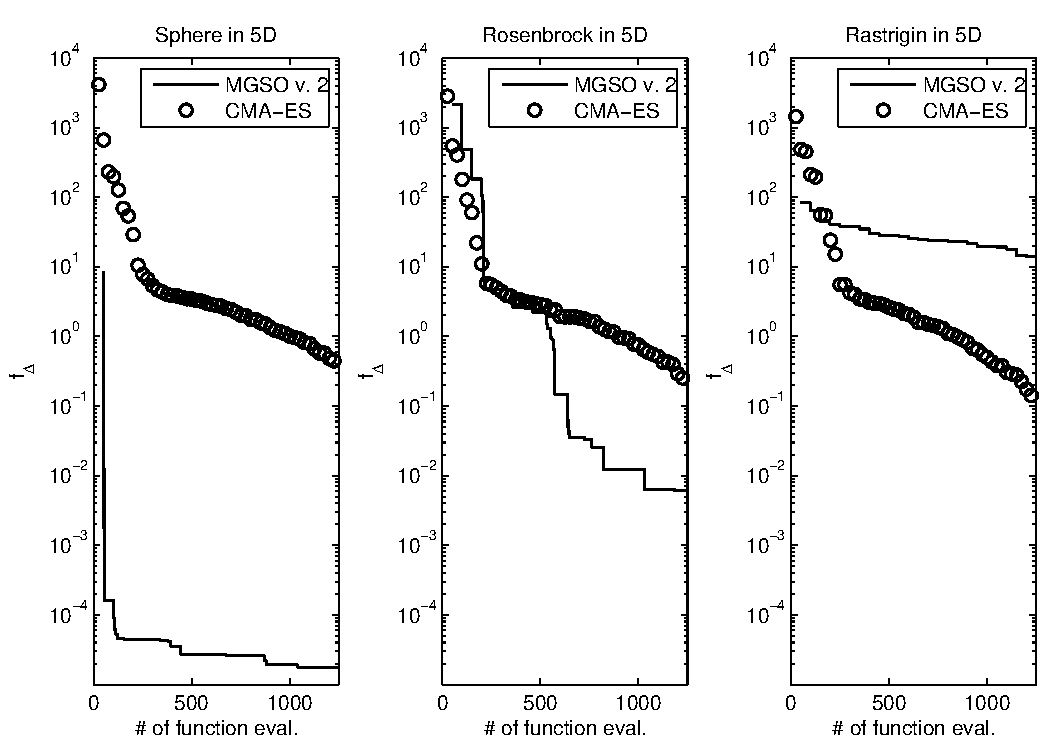
\includegraphics[width=\linewidth]{optim_5D}
  {\small
    \caption{5-D. Medians of the best found function values gathered from 15 runs. The second version of MGSO is compared to CMA-ES.
  \label{fig:optim_5D}
  }
  }
\end{figure}


\begin{figure}
  \centering
  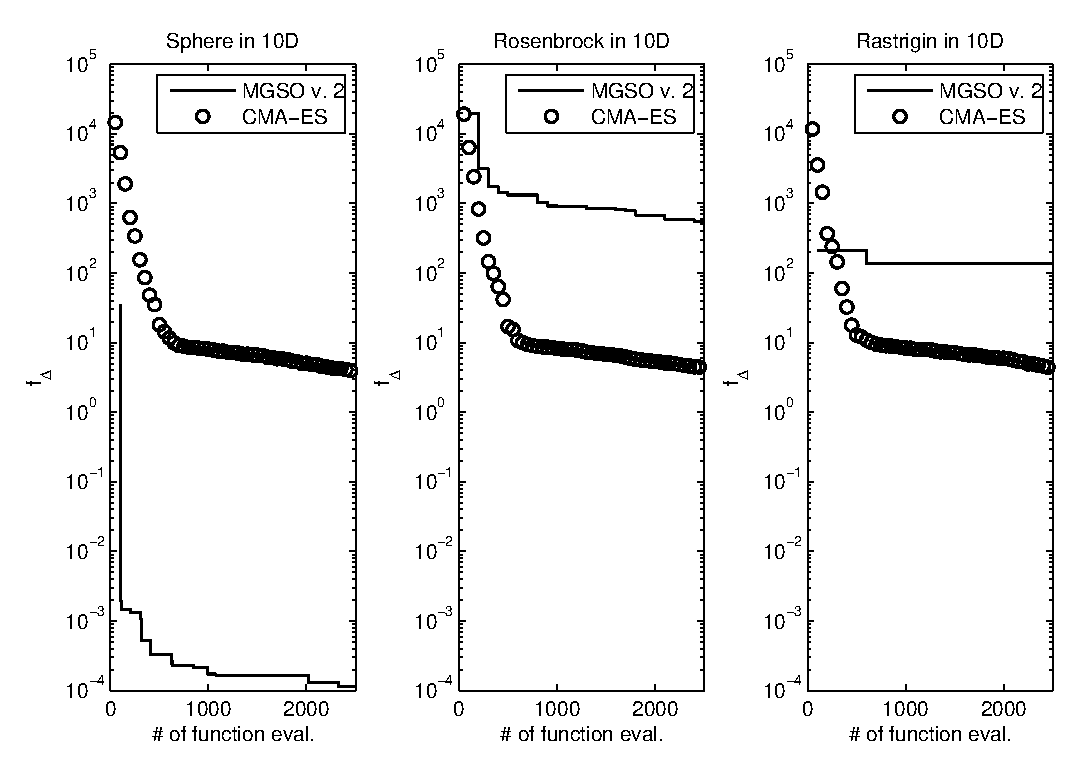
\includegraphics[width=\linewidth]{optim_10D}
  {\small
    % \caption{10-D. Medians of the best found function values gathered from 15 runs on different function instances of the three BBOB functions. The second version of MGSO is compared to CMA-ES.
    \caption{5-D. Medians of the best found function values gathered from 15 runs. The second version of MGSO is compared to CMA-ES.
  \label{fig:optim_10D}
  }
  }
\end{figure}


\subsection{Conclusion}

The Model Guided Sampling Optimization was introduced in more detail. Several improvements of this algorithm was given and much more experimental results than in the last brief work~\cite{bajer_model_2013} were provided. The experiments show that the proposed method can successfully compete with the state-of-the art continuous black-box optimization algorithm CMA-ES in lower dimensions and on easier functions.


% \noindent ==================
% 
% Evolutionary algorithms evolve in parallel a set of candidate solutions (a population) in multiple steps. Every iteration (in evolutionary context called generation) the candidate solutions (individuals) are evaluated with the objective function (so called fitness function). Then, some of these individuals are selected; the better ones are preferred. Finally, the selected individuals are modified or recombined between each other, a new population is created and a new generation starts again.
% 
% \paragraph{Surrogate Modelling.}
% Approximation of the fitness function with some regression model is a common cure for tasks when empirical objective function has to be used. These \textit{surrogate models} simulate behaviour of the original function while being much cheaper and much less time consuming to evaluate. As a surrogate model, any suitable regression model can be used~\cite{hosder2001polynomial,buche2005accelerating,ulmer2005model}.
% 
% In connection with evolutionary optimization, artificial neural networks of the type multilayer perceptrons \cite{jin2005neural} and networks with radial basis functions \cite{zhou2007combining,ong2004surrogate} have been particularly popular. The last mentioned kind of neural networks underlies also the model reported in this paper.





\subsection*{Acknowledgments}

This work was supported by the Czech Science Foundation (GA\v{C}R) grants \hbox{P202/11/1368} and \hbox{13-17187S}, and the Grant Agency of the Charles University (GAUK) \hbox{278511/2011} grant. 

%
% ---- Bibliography ----
%
\bibliography{bajer2013itat}  % sigproc.bib is the name of the Bibliography in this case
\bibliographystyle{abbrv}

% %
% \begin{thebibliography}{5}
% %
% \bibitem {clar:eke}
% Clarke, F., Ekeland, I.:
% Nonlinear oscillations and
% boundary-value problems for Hamiltonian systems.
% Arch. Rat. Mech. Anal. {\bf 78} (1982) 315--333
% 
% \bibitem {clar:eke:2}
% Clarke, F., Ekeland, I.:
% Solutions p\'{e}riodiques, du
% p\'{e}riode donn\'{e}e, des \'{e}quations hamiltoniennes.
% Note CRAS Paris {\bf 287} (1978) 1013--1015
% 
% \bibitem {mich:tar}
% Michalek, R., Tarantello, G.:
% Subharmonic solutions with prescribed minimal
% period for nonautonomous Hamiltonian systems.
% J. Diff. Eq. {\bf 72} (1988) 28--55
% 
% \bibitem {tar}
% Tarantello, G.:
% Subharmonic solutions for Hamiltonian
% systems via a $\bbbz_{p}$ pseudoindex theory.
% Annali di Matematica Pura (to appear)
% 
% \bibitem {rab}
% Rabinowitz, P.:
% On subharmonic solutions of a Hamiltonian system.
% Comm. Pure Appl. Math. {\bf 33} (1980) 609--633
% 
% \end{thebibliography}

\end{document}
